\documentclass[12pt]{article}

\usepackage{fullpage}
\usepackage{amsfonts}
\usepackage{graphicx}
\usepackage{hyperref}
\usepackage{standalone}
\usepackage{amsmath}
\usepackage[margin=1.0in, paperwidth=8.5in]{geometry}
\usepackage{dsfont}
\usepackage{wrapfig}
\usepackage{cite}
\usepackage{relsize}
\usepackage{amssymb}
\usepackage[shortlabels]{enumitem}
\usepackage{IEEEtrantools}
\usepackage{authblk}
\usepackage{setspace}

\begin{document}

\title{Numerical Notes}
\author{}
\date{\today}

\maketitle


\section{Number of modes, N}
Let $L$ be the length of our domain, $\kappa$ be the coefficient of molecular diffusion, $U$ be the RMS velocity for the energy-constrained case, and $\gamma$ be the RMS rate-of-strain for the enstrophy-constrained case. We know that the Batchelor scale is given by 
\begin{equation}
l=\kappa/ U
\end{equation}
for the energy-constrained case or 
\begin{equation}
l=\sqrt{\kappa/\gamma}.
\end{equation}
So we would like the maximum wavenumber to be $k_{max}=(2\pi /L) (N/2) >2\pi/l$. We get the following criteria,
\begin{equation}
N > 2L/l.
\end{equation}
This becomes
\begin{equation}
N > 2L U/\kappa
\end{equation}
for the energy-constrained case or
\begin{equation}
N > 2L \sqrt{\gamma/ \kappa}
\end{equation}
for the enstrophy-constrained case.

\subsection{Boyd's rule-of-thumb}
Estimate the number of wavelengths,$M =L/l$ where $l$ is the smallest scaled needed to be resolved. Then, use the following formula (justified in Boyd, Pg 55)
\begin{equation}
N\geq6+4(M-1)
\end{equation}
So, for the energy case, we have
\begin{equation}
N\geq 6+4\left(\frac{LU}{\kappa}-1\right),
\end{equation}
and for the enstrophy case, we have
\begin{equation}
N\geq 6+4\left(L\sqrt{\frac{\gamma}{\kappa}}-1\right).
\end{equation}



\section{CFL condtion}

Using the CFL condition,
\begin{equation}
h < \frac{ \Delta x}{u} .
\end{equation}
$\Delta x$ is the resolved smallest scale; $\Delta x=\frac{2\pi}{k_{max}} = 2L/N$. $u$ is the velocity scale. For the energy-constrained case, this is simply $u=U$. For the enstrophy-constrained case, this is simply $u=\gamma L$. This condition becomes
\begin{equation}
h < \frac{2L }{U N} 
\end{equation}
for the energy-constrained case or
\begin{equation}
h < \frac{2}{\gamma N} 
\end{equation}
for the enstrophy-constrained case. The above criteria will be used for fixed time-stepping. We will implement RKF45 with adaptive timestepping so that we can have more robust code and maintain stability throughout simulation.

\section{Numerical time integration}
We wish to numerically integrate

\begin{equation}
\frac{\partial \theta }{\partial t} + \mathbf{u}\cdot \nabla \theta = \kappa \Delta \theta
\end{equation}

If we use the following change of variables, 
\begin{equation}
\theta(\mathbf{x},t)=\phi (\mathbf{x},t)e^{-\kappa k^{\star 2}t},
\end{equation}
then we arrive at
\begin{equation}
\frac{\partial \phi }{\partial t} e^{-\kappa k^{\star 2}t}  + \mathbf{u}\cdot \nabla \phi e^{-\kappa k^{\star 2}t}= \kappa \Delta \phi e^{-\kappa k^{\star 2}t} + \kappa k^{\star 2} \phi  e^{-\kappa k^{\star 2}t}.
\end{equation}
This simplifies to 
\begin{equation}
\frac{\partial \phi }{\partial t}   + \mathbf{u}\cdot \nabla \phi = \kappa \Delta \phi  + \kappa k^{\star 2} \phi  .
\end{equation}
Given that our domain is doubly periodic, a natural basis is the set of Fourier functions. We evolve the advection equation in Fourier space. This is given by

\begin{equation}
\label{eq:original_DE}
\frac{d}{d t} \hat{\phi}_{\mathbf{k}} = \mathcal{F}_{\mathbf{k}}(- \mathbf{u}\cdot\nabla \phi) - \kappa( |\mathbf{k}|^{2} - k^{\star 2})\hat{\phi}_{\mathbf{k}}
\end{equation}
for each mode $\mathbf{k}$ where  $\mathcal{F}_{\mathbf{k}}$ is the Fourier transform operator.  Let us define 
\begin{equation}
\Phi_{\mathbf{k}}(t,\hat{\phi})\equiv \mathcal{F}_{\mathbf{k}}(- \mathbf{u}\cdot\nabla \phi) - \kappa( |\mathbf{k}|^{2} - k^{\star 2})\hat{\phi}_{\mathbf{k}}, 
\end{equation}
so that 
\begin{equation}
\frac{d}{d t} \hat{\phi}_{\mathbf{k}}  = \Phi_{
\mathbf{k}}(t,\hat{\phi})
\end{equation}
where $\hat{\phi}$ represents the entire set of $\phi_{\mathbf{k}}$'s. In our current application, $\Phi$ truly does not have explicit time dependence. We include this explicit time dependence as an argument to generalize to potential future applications that may have explicit time dependence.


\subsection{Cash-Karp adaptive time-stepping method}


Now, we implement our time-stepping scheme. We use the embedded Runge-Kutta-Fehlberg 4(5) (RKF45) method with Cash-Karp Parameters.  The fourth-order formula is given by 
\begin{equation}
\label{eq:fourthorder}
\hat{\phi}_{\mathbf{k}}^{j+1 , *}=\hat{\phi}_{\mathbf{k}}^{j, *}+c_{1}^{*}\hat{g}_{\mathbf{k},1}  + c_{2}^{*}\hat{g}_{\mathbf{k},2} + \dots +  c_{6}^{*}\hat{g}_{\mathbf{k},6} + O(h^{5})
\end{equation}
while the fifth-order formula is 
\begin{equation}
\label{eq:fifthorder}
\hat{\phi}_{\mathbf{k}}^{j+1}=\hat{\phi}_{\mathbf{k}}^{j}+c_{1}\hat{g}_{\mathbf{k},1}  + c_{2}\hat{g}_{\mathbf{k},2} + \dots +  c_{6}\hat{g}_{\mathbf{k},6}  + O(h^{6})
\end{equation}
where 
\begin{subequations}
	\begin{align}
		\hat{g}_{\mathbf{k},1} & = h \hat{\Phi}_{\mathbf{k}}(t^{j} \, , \, \hat{\phi}^{j}_{\mathbf{k}}) \\
		\hat{g}_{\mathbf{k},2} & = h \hat{\Phi}_{\mathbf{k}}(t^{j}+a_{2}h \, , \, \hat{\phi}^{j}_{\mathbf{k}} + b_{21}\hat{g}_{\mathbf{k},1}  ) \\
		\notag
		\vdots \\
		\hat{g}_{\mathbf{k},6} & = h \hat{\Phi}_{\mathbf{k}}(t^{j}+a_{6}h \, , \, \hat{\phi}^{j}_{\mathbf{k}} + b_{61}\hat{g}_{\mathbf{k},1}  + \dots +    b_{65}\hat{g}_{\mathbf{k},5} ) .
	\end{align}
\end{subequations}
The error estimate is given by the magnitude of the complex difference between (\ref{eq:fifthorder}) and (\ref{eq:fourthorder}),
\begin{equation}
\epsilon_{\mathbf{k}}^{j}\equiv |\hat{\phi}_{\mathbf{k}}^{j+1}-\hat{\phi}_{\mathbf{k}}^{j+1,*}| = \left|\sum_{i=1}^{6} (c_{i}-c_{i}^{*})\hat{g
}_{\mathbf{k},i} \right| .
\end{equation}
\begin{figure*}
	\centering
	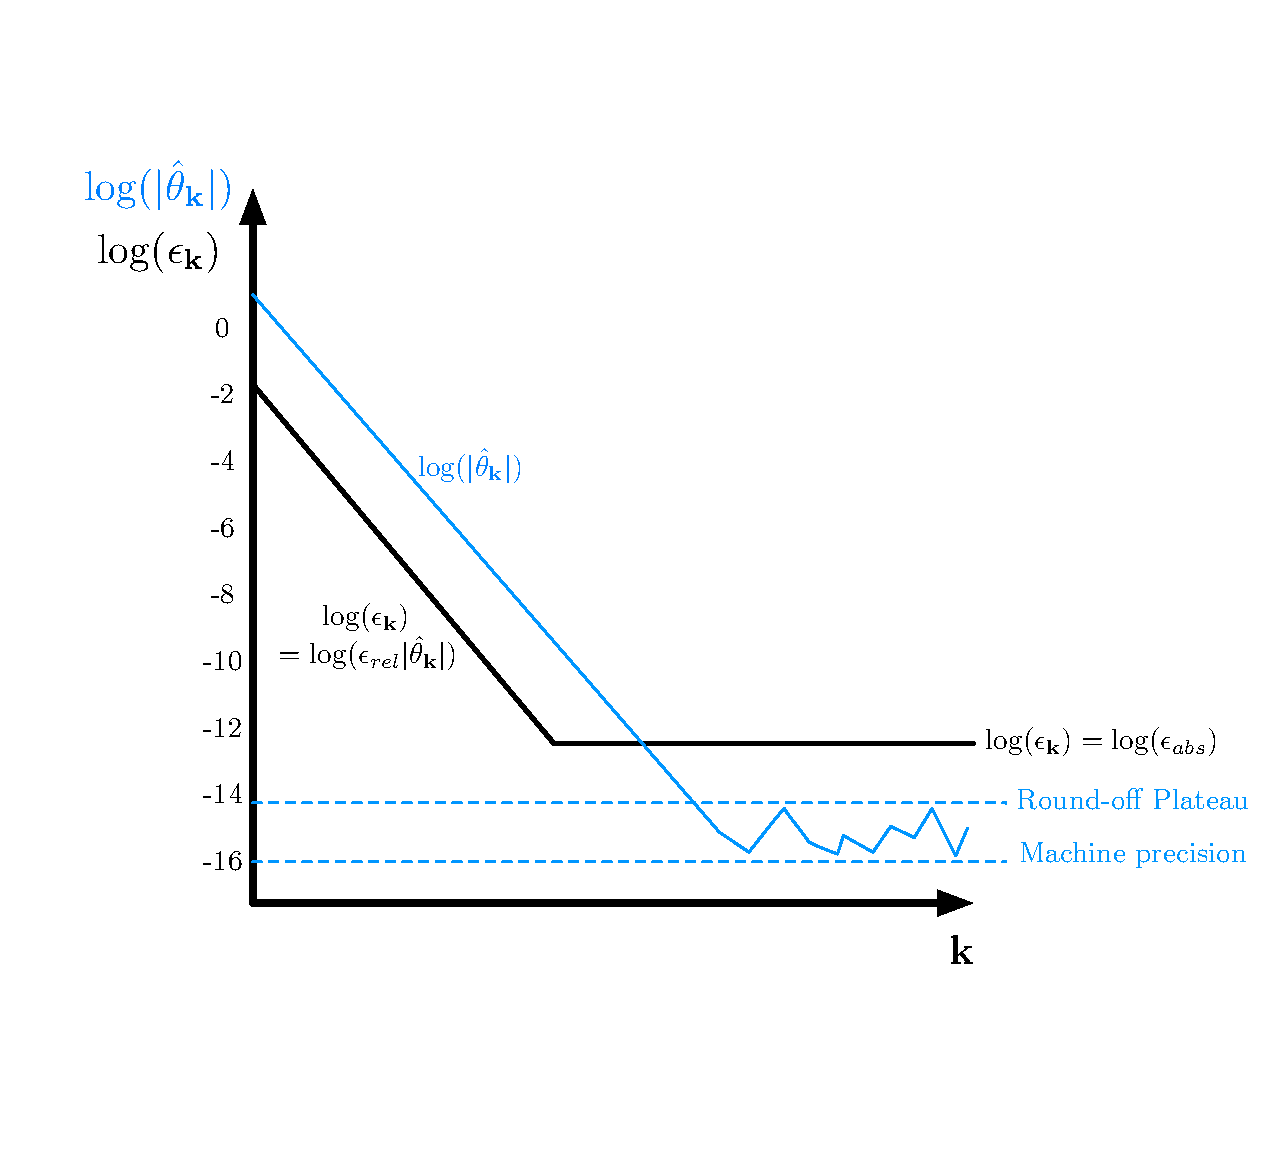
\includegraphics[width=0.6\textwidth]{spectrum_errors.eps}
	\caption{Error analysis.}
	\label{fig:spectrum_errors}
\end{figure*}
We will accept a solution if 
\begin{equation}
\label{eq:acceptance_criteria}
\epsilon_{\mathbf{k}}^{j}< \epsilon_{\mathbf{k},d} =  \epsilon_{abs}
\end{equation}
for all $\mathbf{k}$. Note we must choose  $\epsilon_{abs}$ greater than machine round-off error $\epsilon_{m} \approx 10^{-16}$.  Note that the global absolute error  $\sigma_{\mathbf{k}}$ at the time $T$ is bounded by:
\begin{equation}
\label{eq:global_error_estimate}
\sigma_{\mathbf{k}}=\sum_{j} \epsilon^{j}_{\mathbf{k}} \leq \sum_{j} \epsilon_{abs}  =\epsilon_{abs} M
\end{equation}
where $M$ is the number of time steps. If $\sigma_{d}$ is the desired global absolute error at the end  time $T$, then we would like to set $\epsilon_{abs} M = \sigma_{d}$.  Since this is an adaptive time-stepping scheme, $M$ can vary across simulations, instead we choose $\epsilon_{abs}=\sigma_{d}h^{j}/T$ to achieve the same result. Substituting this relation into $\ref{eq:global_error_estimate}$, we see that $\sigma_{\mathbf{k}}\leq \sigma_{d}$ as desired. We then pick out the mode $\mathbf{k}^{*}$ that violates criteria (\ref{eq:acceptance_criteria}) `the most' defined by
\begin{equation}
\mathbf{k}^{*}=argmax_{\mathbf{k}} \epsilon_{\mathbf{k}}-\epsilon_{\mathbf{k},d}.
\end{equation}
Since (\ref{eq:fourthorder}) is fourth-order, we know the error estimate is approximately $\epsilon_{\mathbf{k}^{*}}=d h^{5}$ for some constant $d$. Then this gives us the constant $d= \epsilon_{\mathbf{k}^{*}}/h^5$. Thus, we can then use this to chose a new step size $h_{new}$ to achieve a desired  error $\epsilon_{d}$ by 
\begin{equation}
h_{new}=h \left(\frac{\epsilon_{\mathbf{k}^{*},d}}{\epsilon_{\mathbf{k}^{*}}}\right)^{1/5}.
\end{equation}
It is common to modify this relation by introducing a safety parameter $\beta $ that is slightly less than 1 (=0.8 or 0.9) and conditionally changing the exponent. The recommended prescription is 
\begin{eqnarray}
h := \beta h \left(\frac{\epsilon_{\mathbf{k}^{*},d}}{\epsilon_{\mathbf{k}^{*}}}\right)^{1/5} \, ,\, \epsilon \geq \epsilon_{d} \\
h := \beta h \left(\frac{\epsilon_{\mathbf{k}^{*},d}}{\epsilon_{\mathbf{k}^{*}}}\right)^{1/4}\, ,\, \epsilon <\epsilon_{d} .
\end{eqnarray}
\begin{figure*}
	\centering
	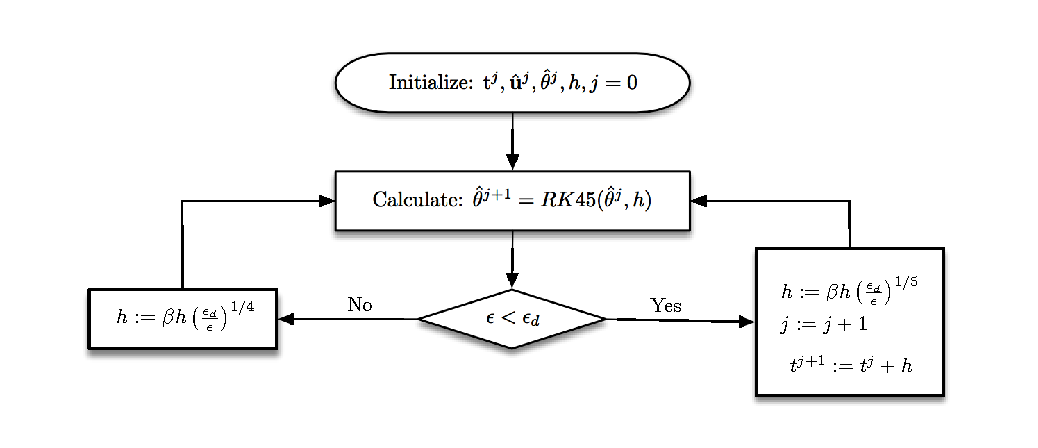
\includegraphics[width=1.0\textwidth]{RK45.eps}
	\caption{RKF45 flow diagram for adaptive time-stepping.}
	\label{fig:RKF45}
\end{figure*}
The adaptive time-stepping scheme in RKF45 is shown in figure \ref{fig:RKF45}. 

Since the step decision is based on the error scaling with $h$ of the fourth-order formula, we will use the fourth-order formula as our final update: $\hat{\theta}_{\mathbf{k}}(t^{j+1})=\hat{\theta}_{\mathbf{k}}^{j+1,*}$.

\end{document}